\documentclass{article}
\usepackage{fullpage,booktabs,graphicx,hyperref,float,array}
% generated by grnbench report from result files - do not edit
\newcommand{\gbCiHighAuprcRatioAutoGrnboostTwoMotifVsGrnboostTwo}{+0.153}
\newcommand{\gbCiHighAuprcRatioAutoRegdiffusionMotifVsRegdiffusion}{+0.237}
\newcommand{\gbCiHighAuprcRatioBaselineGrnboostTwoMotifVsGrnboostTwo}{+0.149}
\newcommand{\gbCiHighAuprcRatioBaselineRegdiffusionMotifVsRegdiffusion}{+0.236}
\newcommand{\gbCiHighEprAutoGrnboostTwoMotifVsGrnboostTwo}{+0.739}
\newcommand{\gbCiHighEprAutoRegdiffusionMotifVsRegdiffusion}{+0.191}
\newcommand{\gbCiHighEprBaselineGrnboostTwoMotifVsGrnboostTwo}{+0.673}
\newcommand{\gbCiHighEprBaselineRegdiffusionMotifVsRegdiffusion}{+0.214}
\newcommand{\gbCiLowAuprcRatioAutoGrnboostTwoMotifVsGrnboostTwo}{+0.108}
\newcommand{\gbCiLowAuprcRatioAutoRegdiffusionMotifVsRegdiffusion}{+0.132}
\newcommand{\gbCiLowAuprcRatioBaselineGrnboostTwoMotifVsGrnboostTwo}{+0.110}
\newcommand{\gbCiLowAuprcRatioBaselineRegdiffusionMotifVsRegdiffusion}{+0.138}
\newcommand{\gbCiLowEprAutoGrnboostTwoMotifVsGrnboostTwo}{+0.473}
\newcommand{\gbCiLowEprAutoRegdiffusionMotifVsRegdiffusion}{-0.197}
\newcommand{\gbCiLowEprBaselineGrnboostTwoMotifVsGrnboostTwo}{+0.422}
\newcommand{\gbCiLowEprBaselineRegdiffusionMotifVsRegdiffusion}{-0.201}
\newcommand{\gbDiffAuprcRatioAutoGrnboostTwoMotifVsGrnboostTwo}{+0.130}
\newcommand{\gbDiffAuprcRatioAutoRegdiffusionMotifVsRegdiffusion}{+0.184}
\newcommand{\gbDiffAuprcRatioBaselineGrnboostTwoMotifVsGrnboostTwo}{+0.129}
\newcommand{\gbDiffAuprcRatioBaselineRegdiffusionMotifVsRegdiffusion}{+0.187}
\newcommand{\gbDiffEprAutoGrnboostTwoMotifVsGrnboostTwo}{+0.606}
\newcommand{\gbDiffEprAutoRegdiffusionMotifVsRegdiffusion}{-0.003}
\newcommand{\gbDiffEprBaselineGrnboostTwoMotifVsGrnboostTwo}{+0.548}
\newcommand{\gbDiffEprBaselineRegdiffusionMotifVsRegdiffusion}{+0.006}
\newcommand{\gbFamilyAuprcRatioAuto}{4}
\newcommand{\gbFamilyAuprcRatioBaseline}{4}
\newcommand{\gbFamilyEprAuto}{4}
\newcommand{\gbFamilyEprBaseline}{4}
\newcommand{\gbMeanAuprcRatioAutoGrnboostTwo}{1.102}
\newcommand{\gbMeanAuprcRatioAutoGrnboostTwoMotif}{1.232}
\newcommand{\gbMeanAuprcRatioAutoRegdiffusion}{1.416}
\newcommand{\gbMeanAuprcRatioAutoRegdiffusionMotif}{1.600}
\newcommand{\gbNAuprcRatioAutoGrnboostTwoMotifVsGrnboostTwo}{20}
\newcommand{\gbNAuprcRatioAutoRegdiffusionMotifVsRegdiffusion}{19}
\newcommand{\gbNAuprcRatioBaselineGrnboostTwoMotifVsGrnboostTwo}{20}
\newcommand{\gbNAuprcRatioBaselineRegdiffusionMotifVsRegdiffusion}{19}
\newcommand{\gbNAutoGrnboostTwo}{20}
\newcommand{\gbNAutoGrnboostTwoMotif}{20}
\newcommand{\gbNAutoRegdiffusion}{19}
\newcommand{\gbNAutoRegdiffusionMotif}{19}
\newcommand{\gbNDatasets}{20}
\newcommand{\gbNEprAutoGrnboostTwoMotifVsGrnboostTwo}{20}
\newcommand{\gbNEprAutoRegdiffusionMotifVsRegdiffusion}{19}
\newcommand{\gbNEprBaselineGrnboostTwoMotifVsGrnboostTwo}{20}
\newcommand{\gbNEprBaselineRegdiffusionMotifVsRegdiffusion}{19}
\newcommand{\gbPHolmAuprcRatioAutoGrnboostTwoMotifVsGrnboostTwo}{3.6e-10}
\newcommand{\gbPHolmAuprcRatioAutoRegdiffusionMotifVsRegdiffusion}{1.2e-06}
\newcommand{\gbPHolmAuprcRatioBaselineGrnboostTwoMotifVsGrnboostTwo}{4.8e-11}
\newcommand{\gbPHolmAuprcRatioBaselineRegdiffusionMotifVsRegdiffusion}{3.7e-07}
\newcommand{\gbPHolmEprAutoGrnboostTwoMotifVsGrnboostTwo}{2.2e-08}
\newcommand{\gbPHolmEprAutoRegdiffusionMotifVsRegdiffusion}{1.000}
\newcommand{\gbPHolmEprBaselineGrnboostTwoMotifVsGrnboostTwo}{4.4e-08}
\newcommand{\gbPHolmEprBaselineRegdiffusionMotifVsRegdiffusion}{1.000}
\newcommand{\gbPHolmRevAuprcRatioAutoGrnboostTwoMotifVsGrnboostTwo}{1.000}
\newcommand{\gbPHolmRevAuprcRatioAutoRegdiffusionMotifVsRegdiffusion}{1.000}
\newcommand{\gbPHolmRevAuprcRatioBaselineGrnboostTwoMotifVsGrnboostTwo}{1.000}
\newcommand{\gbPHolmRevAuprcRatioBaselineRegdiffusionMotifVsRegdiffusion}{1.000}
\newcommand{\gbPHolmRevEprAutoGrnboostTwoMotifVsGrnboostTwo}{1.000}
\newcommand{\gbPHolmRevEprAutoRegdiffusionMotifVsRegdiffusion}{1.000}
\newcommand{\gbPHolmRevEprBaselineGrnboostTwoMotifVsGrnboostTwo}{1.000}
\newcommand{\gbPHolmRevEprBaselineRegdiffusionMotifVsRegdiffusion}{1.000}

\title{EXP-20260926-LM-1: Confirmatory - does the motif prior lift RegDiffusion and GRNBoost2 on real data?}
\author{grnbench report generated from EXP-20260926-LM-1}
\date{}
\begin{document}
\maketitle
\section*{Status}
Experiment EXP-20260926-LM-1, type: confirmatory. Record status: done (2026-09-27; Slurm job 670902, COMPLETED 0:0 in 1 h 10 min, 20/20 datasets, 0 task errors; 8 workers on gnode01, peak memory of the batch step 11.7 GiB of the 32 GB requested). Reproduced by: nobody yet.
\section{Configuration summary}
\begin{table}[H]\centering\small
\caption{Configuration of the run, from the experiment record and the run folder.}
\begin{tabular}{p{0.3\linewidth}p{0.62\linewidth}}\toprule
experiment & EXP-20260926-LM-1 \\
type & **confirmatory** (pre-registration = the commit that adds this file, pushed before any of the four models below was run on any dataset of this list) \\
owner & LM (agent-run)   issue: \#10   registered: 2026-09-26 \\
datasets (rows) & 20 \\
models & grnboost2, grnboost2\_motif, regdiffusion, regdiffusion\_motif \\
arms & auto, baseline \\
code & branch lm/exp-hpc-motif-models after merging main with PR \#11 (issue \#6: batches under 100 cells are pooled for scrublet, so the 4 LM-2 datasets that fell back to the heuristic now get scrublet; this changes their processed data relative to LM-2, which is one more reason the comparison with LM-2 is descriptive only). The job copies GIT\_COMMIT (written by hpc/hpc.sh sync) to the results folder as CODE\_COMMIT; that commit must be clean. \\
code commit (run folder) & 84f28e1edfdee819cce4e5323c719cc59a32b1fc \\
environment & conda env grnbench on the cluster, Python 3.11, requirements/lock-py311.txt plus the RegDiffusion line of its header (regdiffusion 0.2.3, torch 2.14.0 CPU) via WITH\_TORCH=1 bash hpc/setup\_env.sh. \\
machine & Bocconi HPC, partition/QOS stud, 1 job, 8 CPUs (8 dataset workers, one thread each), 32 GB. Expected cost: RegDiffusion took 808 s per dataset and arm on the laptop in LM-1; with --keep-artifacts both arms are scored, so about 40 RegDiffusion fits plus screening, roughly 3-6 h on 8 single-threaded workers. \\
seeds & reference split seed 0 (screen.split\_reference), cell subsample seed 0 (at most 3,000 cells per context, MAX\_SCORE\_CELLS), scrublet seed 0, RegDiffusion seed 0 (1,000 steps, CPU), GRNBoost2 seed 42 (the adapter defaults); regulators = the 150 TFs with most reference targets in the data (MAX\_TFS). \\
run folder & benchmarks/results/EXP-20260926-LM-1 \\
generated & 2026-09-27 08:34 \\
\bottomrule\end{tabular}\end{table}

\section{Methods}
\begin{description}
\item[type] **confirmatory** (pre-registration = the commit that adds this file, pushed before any of the four models below was run on any dataset of this list)
\item[hypothesis] co-primary, directional. H1: regdiffusion\_motif (RegDiffusion edges rank-producted with the cisTarget motif prior) recovers the CollecTRI evaluation half better than regdiffusion alone. H2: grnboost2\_motif recovers it better than grnboost2 alone.
\item[primary endpoint] AUPRC ratio (AUPRC / prevalence; 1 = random) on the CollecTRI evaluation half, **auto** pipeline arm (the engine's screened choice), mean over contexts within a dataset.
\item[secondary endpoints (reported, not used for h1/h2)] EPR; the baseline pipeline arm; each model's mean AUPRC ratio against random (1.0), descriptive only.
\item[unit of analysis] dataset. Planned n = 20; analysed n = datasets with a score for both members of a pair (printed per pair by the report).
\item[datasets] the 20 CELLxGENE datasets of EXP-20260925-LM-2 (experiments/EXP-20260925-LM-2.datasets.tsv; sha256 of every data.h5ad and truth.json in experiments/datasets.tsv). Why not fresh data: (1) none of the four models has ever been scored on them (the exploratory estimates above come from 12 other datasets); (2) their bytes are pinned by sha256, so the cluster copy is checked, not trusted; (3) the same datasets make these results directly comparable with the Pearson results of LM-2 (descriptive only, no test across experiments). What this costs: the motif prior and the pipeline choices on these datasets were already seen in LM-2 with Pearson, so the set is not blind to "the motif prior helps on these data". A fresh-set rerun would remove that.
\item[exclusion rules (fixed now)] (a) a dataset whose download fails or whose sha256 does not match experiments/datasets.tsv is replaced by nobody and reported as missing (for truth.json a difference in line endings only is accepted, data\_manifest.py --check reports it as ok-eol); (b) datasets with fewer than 50 reference edges among their genes are not scored (MIN\_REFERENCE\_EDGES); (c) a dataset where a model errors is dropped from the pairs involving that model only, and reported; (d) a dataset still unfinished after the job and one resubmission of the same commit (resource limits: TIMEOUT or out of memory) is reported as missing; (e) no other exclusion, no outlier removal.
\item[comparison family] real\_bench.DECLARED\_PAIRS restricted to the models run = \{(regdiffusion\_motif, regdiffusion), (grnboost2\_motif, grnboost2)\}, both directions = 4 directed hypotheses per metric and arm.
\item[test] paired t over datasets, two-sided per direction, via compare\_units for each pair (95\% interval of the mean paired difference), Holm over the 4 directed hypotheses of the AUPRC ratio / auto family, alpha 0.05. For each of H1, H2: **supported** if p\_Holm(motif > plain) < 0.05; **refuted** if p\_Holm(plain > motif) < 0.05; otherwise inconclusive (not evidence of equality). Holm over the family already accounts for testing two co-primary hypotheses.
\item[seeds] reference split seed 0 (screen.split\_reference), cell subsample seed 0 (at most 3,000 cells per context, MAX\_SCORE\_CELLS), scrublet seed 0, RegDiffusion seed 0 (1,000 steps, CPU), GRNBoost2 seed 42 (the adapter defaults); regulators = the 150 TFs with most reference targets in the data (MAX\_TFS).
\item[models] regdiffusion, regdiffusion\_motif, grnboost2, grnboost2\_motif (exactly these four).
\item[code] branch lm/exp-hpc-motif-models after merging main with PR \#11 (issue \#6: batches under 100 cells are pooled for scrublet, so the 4 LM-2 datasets that fell back to the heuristic now get scrublet; this changes their processed data relative to LM-2, which is one more reason the comparison with LM-2 is descriptive only). The job copies GIT\_COMMIT (written by hpc/hpc.sh sync) to the results folder as CODE\_COMMIT; that commit must be clean.
\item[environment] conda env grnbench on the cluster, Python 3.11, requirements/lock-py311.txt plus the RegDiffusion line of its header (regdiffusion 0.2.3, torch 2.14.0 CPU) via WITH\_TORCH=1 bash hpc/setup\_env.sh.
\item[machine] Bocconi HPC, partition/QOS stud, 1 job, 8 CPUs (8 dataset workers, one thread each), 32 GB. Expected cost: RegDiffusion took 808 s per dataset and arm on the laptop in LM-1; with --keep-artifacts both arms are scored, so about 40 RegDiffusion fits plus screening, roughly 3-6 h on 8 single-threaded workers.
\item[models scored] grnboost2, grnboost2\_motif, regdiffusion, regdiffusion\_motif
\end{description}

\section{Results}
\subsection{Primary comparison}
\paragraph{Pre-registered primary hypothesis.} regdiffusion\_motif $>$ regdiffusion on AUPRC ratio, auto pipeline. Mean paired difference \gbDiffAuprcRatioAutoRegdiffusionMotifVsRegdiffusion{} (95\% interval \gbCiLowAuprcRatioAutoRegdiffusionMotifVsRegdiffusion{} to \gbCiHighAuprcRatioAutoRegdiffusionMotifVsRegdiffusion{}), n = \gbNAuprcRatioAutoRegdiffusionMotifVsRegdiffusion{} datasets, paired t, Holm over \gbFamilyAuprcRatioAuto{} directed hypotheses: $p_{\mathrm{Holm}}$ = \gbPHolmAuprcRatioAutoRegdiffusionMotifVsRegdiffusion{}. Verdict by the rule fixed in the record: \textbf{supported}.
\paragraph{Pre-registered primary hypothesis.} grnboost2\_motif $>$ grnboost2 on AUPRC ratio, auto pipeline. Mean paired difference \gbDiffAuprcRatioAutoGrnboostTwoMotifVsGrnboostTwo{} (95\% interval \gbCiLowAuprcRatioAutoGrnboostTwoMotifVsGrnboostTwo{} to \gbCiHighAuprcRatioAutoGrnboostTwoMotifVsGrnboostTwo{}), n = \gbNAuprcRatioAutoGrnboostTwoMotifVsGrnboostTwo{} datasets, paired t, Holm over \gbFamilyAuprcRatioAuto{} directed hypotheses: $p_{\mathrm{Holm}}$ = \gbPHolmAuprcRatioAutoGrnboostTwoMotifVsGrnboostTwo{}. Verdict by the rule fixed in the record: \textbf{supported}.

\subsection{Performance per model, across datasets}
\begin{table}[H]\centering\small
\caption{Reference recovery per model (CollecTRI evaluation half; AUPRC ratio, 1 = random). Unit = dataset; n per model shown.}
\begin{tabular}{lrrrr}\toprule
model & n & mean (auto) & median (auto) & mean (baseline) \\ \midrule
regdiffusion\_motif & 19 & 1.600 & 1.566 & 1.599 \\
regdiffusion & 19 & 1.416 & 1.330 & 1.412 \\
grnboost2\_motif & 20 & 1.232 & 1.223 & 1.237 \\
grnboost2 & 20 & 1.102 & 1.087 & 1.108 \\
\bottomrule\end{tabular}\end{table}

\subsection{Performance per dataset}
\begin{table}[H]\centering\scriptsize
\caption{AUPRC ratio per dataset, auto pipeline (1 = random); the unit of analysis.}
\resizebox{\linewidth}{!}{\begin{tabular}{lrrrr}\toprule
dataset & regdiffusion\_motif & regdiffusion & grnboost2\_motif & grnboost2 \\ \midrule
10x-3-v2\_\_homo-sapiens\_\_entorhinal-cortex\_\_06b91 & n/a & n/a & 1.20 & 1.05 \\
10x-3-v2\_\_homo-sapiens\_\_peripheral-zone-of-prost & 1.34 & 1.22 & 1.17 & 1.07 \\
10x-3-v2\_\_homo-sapiens\_\_superior-frontal-gyrus\_\_ & 1.81 & 1.54 & 1.16 & 1.05 \\
10x-3-v2\_\_mus-musculus\_\_spinal-cord\_\_8ef59750 & 1.52 & 1.17 & 1.20 & 1.07 \\
10x-3-v3\_\_homo-sapiens\_\_primary-motor-cortex\_\_9b & 1.31 & 1.12 & 1.13 & 1.03 \\
10x-3-v3\_\_homo-sapiens\_\_prostate-gland\_\_20de8570 & 1.67 & 1.46 & 1.28 & 1.14 \\
10x-3-v3\_\_homo-sapiens\_\_respiratory-airway\_\_eec8 & 1.92 & 1.77 & 1.33 & 1.16 \\
10x-3-v3\_\_mus-musculus\_\_autopod-skin\_\_389b1fd4 & 1.67 & 1.50 & 1.29 & 1.12 \\
10x-3-v3\_\_mus-musculus\_\_epididymal-fat-pad\_\_e252 & 1.45 & 1.23 & 1.16 & 1.06 \\
10x-5-v1\_\_homo-sapiens\_\_lung\_\_62315937 & 1.61 & 1.28 & 1.31 & 1.09 \\
10x-5-v1\_\_homo-sapiens\_\_lung\_\_7b3368a5 & 1.95 & 1.55 & 1.33 & 1.13 \\
10x-multiome\_\_homo-sapiens\_\_brain\_\_bdc7e498 & 1.57 & 1.36 & 1.23 & 1.13 \\
10x-multiome\_\_homo-sapiens\_\_cranial-neural-crest & 1.33 & 1.33 & 1.10 & 1.07 \\
cel-seq2\_\_homo-sapiens\_\_bronchial-mucosa\_\_d2bc27 & 2.02 & 1.79 & 1.41 & 1.22 \\
cel-seq2\_\_homo-sapiens\_\_pancreas\_\_b07e5164 & 1.38 & 1.26 & 1.17 & 1.07 \\
patch-seq\_\_mus-musculus\_\_primary-motor-cortex\_\_3 & 1.45 & 1.31 & 1.21 & 1.13 \\
patch-seq\_\_mus-musculus\_\_primary-motor-cortex\_\_b & 1.49 & 1.25 & 1.27 & 1.08 \\
smart-seq2\_\_homo-sapiens\_\_cerebral-cortex\_\_774c1 & 1.38 & 1.33 & 1.14 & 1.07 \\
smart-seq2\_\_mus-musculus\_\_diaphragm\_\_cbd62079 & 1.62 & 1.62 & 1.28 & 1.15 \\
smart-seq2\_\_mus-musculus\_\_kidney\_\_524179b0 & 1.89 & 1.80 & 1.27 & 1.13 \\
\midrule
mean & 1.60 & 1.42 & 1.23 & 1.10 \\
median & 1.57 & 1.33 & 1.22 & 1.09 \\
SD & 0.23 & 0.21 & 0.08 & 0.05 \\
\bottomrule\end{tabular}}\end{table}

\subsection{Comparative summary: declared comparisons}
\begin{table}[H]\centering\small
\caption{Declared comparisons, AUPRC ratio, auto pipeline: paired t over datasets (compare\_units), two-sided per direction, Holm over 4 directed hypotheses; 95\% interval of the mean paired difference.}
\begin{tabular}{llrrlrrl}\toprule
A & B & n & mean A$-$B & 95\% interval & $p_{A>B}$ Holm & $p_{B>A}$ Holm & supported \\ \midrule
grnboost2\_motif & grnboost2 & 20 & +0.130 & [+0.108, +0.153] & 3.6e-10 & 1.000 & grnboost2\_motif \\
regdiffusion\_motif & regdiffusion & 19 & +0.184 & [+0.132, +0.237] & 1.2e-06 & 1.000 & regdiffusion\_motif \\
\bottomrule\end{tabular}\end{table}

\begin{table}[H]\centering\small
\caption{Declared comparisons, AUPRC ratio, baseline pipeline: paired t over datasets (compare\_units), two-sided per direction, Holm over 4 directed hypotheses; 95\% interval of the mean paired difference.}
\begin{tabular}{llrrlrrl}\toprule
A & B & n & mean A$-$B & 95\% interval & $p_{A>B}$ Holm & $p_{B>A}$ Holm & supported \\ \midrule
grnboost2\_motif & grnboost2 & 20 & +0.129 & [+0.110, +0.149] & 4.8e-11 & 1.000 & grnboost2\_motif \\
regdiffusion\_motif & regdiffusion & 19 & +0.187 & [+0.138, +0.236] & 3.7e-07 & 1.000 & regdiffusion\_motif \\
\bottomrule\end{tabular}\end{table}

\begin{table}[H]\centering\small
\caption{Declared comparisons, EPR, auto pipeline: paired t over datasets (compare\_units), two-sided per direction, Holm over 4 directed hypotheses; 95\% interval of the mean paired difference.}
\begin{tabular}{llrrlrrl}\toprule
A & B & n & mean A$-$B & 95\% interval & $p_{A>B}$ Holm & $p_{B>A}$ Holm & supported \\ \midrule
grnboost2\_motif & grnboost2 & 20 & +0.606 & [+0.473, +0.739] & 2.2e-08 & 1.000 & grnboost2\_motif \\
regdiffusion\_motif & regdiffusion & 19 & -0.003 & [-0.197, +0.191] & 1.000 & 1.000 & unresolved \\
\bottomrule\end{tabular}\end{table}

\begin{table}[H]\centering\small
\caption{Declared comparisons, EPR, baseline pipeline: paired t over datasets (compare\_units), two-sided per direction, Holm over 4 directed hypotheses; 95\% interval of the mean paired difference.}
\begin{tabular}{llrrlrrl}\toprule
A & B & n & mean A$-$B & 95\% interval & $p_{A>B}$ Holm & $p_{B>A}$ Holm & supported \\ \midrule
grnboost2\_motif & grnboost2 & 20 & +0.548 & [+0.422, +0.673] & 4.4e-08 & 1.000 & grnboost2\_motif \\
regdiffusion\_motif & regdiffusion & 19 & +0.006 & [-0.201, +0.214] & 1.000 & 1.000 & unresolved \\
\bottomrule\end{tabular}\end{table}

\section{Visualizations and explainability}
\begin{figure}[H]\centering
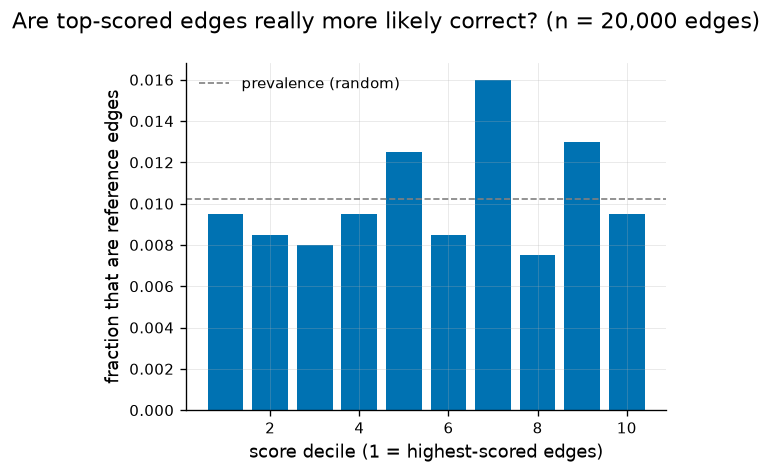
\includegraphics[width=0.85\linewidth]{../viz/calibration_cxg__10x-3-v2__homo-sapiens__entorhinal-cortex__06b91002.png}
\caption{-   (n = 20000 edges) - built from  grnboost2.tsv.gz}
\end{figure}
\begin{figure}[H]\centering
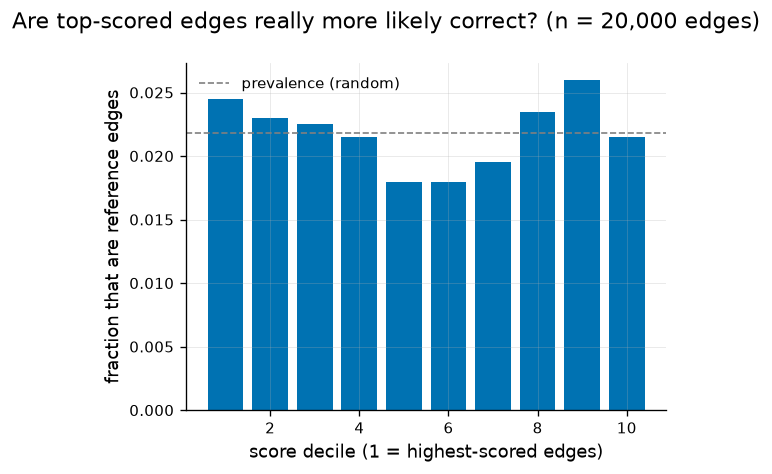
\includegraphics[width=0.85\linewidth]{../viz/calibration_cxg__10x-3-v2__homo-sapiens__peripheral-zone-of-prostate__df287f8d.png}
\caption{-   (n = 20000 edges) - built from  grnboost2.tsv.gz}
\end{figure}
\begin{figure}[H]\centering
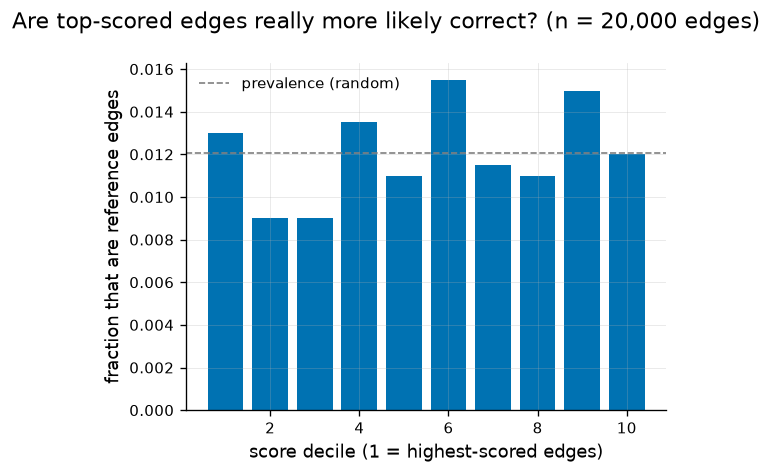
\includegraphics[width=0.85\linewidth]{../viz/calibration_cxg__10x-3-v2__homo-sapiens__superior-frontal-gyrus__b94e3bdf.png}
\caption{-   (n = 20000 edges) - built from  grnboost2.tsv.gz}
\end{figure}
\begin{figure}[H]\centering
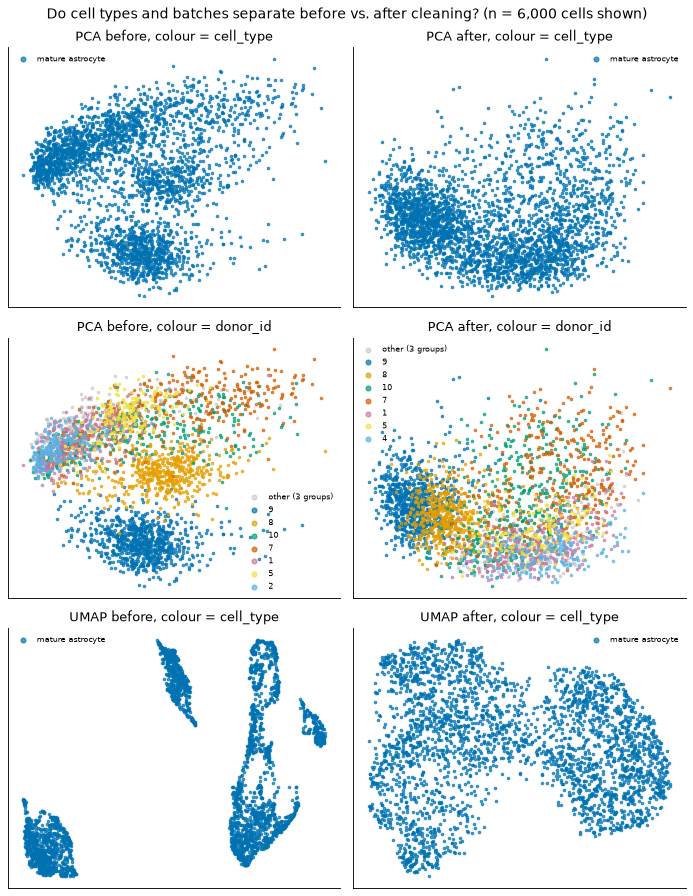
\includegraphics[width=0.85\linewidth]{../viz/embed_cxg__10x-3-v2__homo-sapiens__entorhinal-cortex__06b91002.png}
\caption{-   (n = 5500 cells) - built from  tasks.json (raw data)}
\end{figure}
\begin{figure}[H]\centering
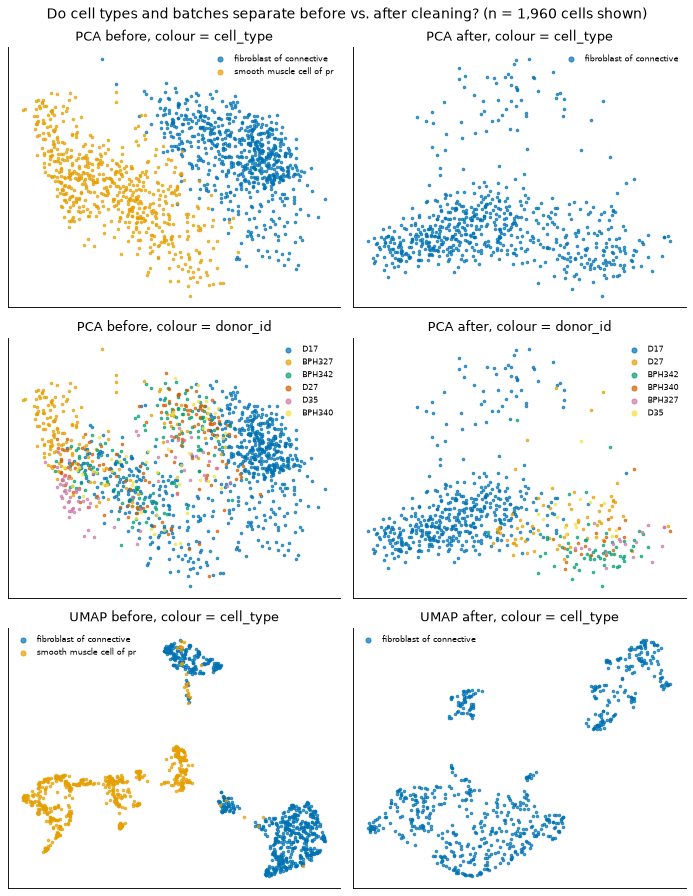
\includegraphics[width=0.85\linewidth]{../viz/embed_cxg__10x-3-v2__homo-sapiens__peripheral-zone-of-prostate__df287f8d.png}
\caption{-   (n = 1295 cells) - built from  tasks.json (raw data)}
\end{figure}
\begin{figure}[H]\centering
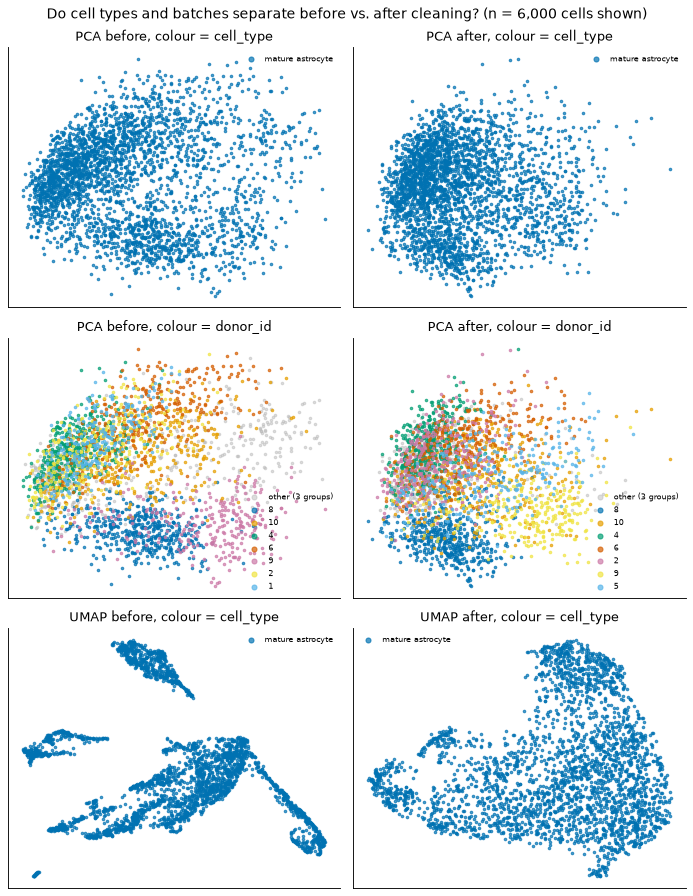
\includegraphics[width=0.85\linewidth]{../viz/embed_cxg__10x-3-v2__homo-sapiens__superior-frontal-gyrus__b94e3bdf.png}
\caption{-   (n = 5970 cells) - built from  tasks.json (raw data)}
\end{figure}
\begin{figure}[H]\centering
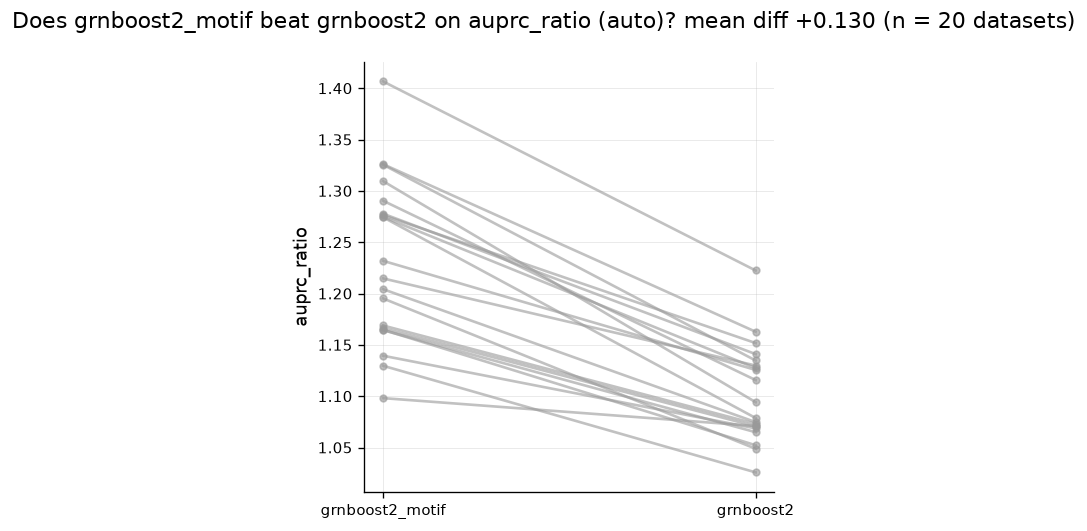
\includegraphics[width=0.85\linewidth]{../viz/lift_grnboost2_motif_vs_grnboost2.png}
\caption{-   (n = 20 datasets) - built from  rows/ .json (grnboost2\_motif vs grnboost2)}
\end{figure}
\begin{figure}[H]\centering
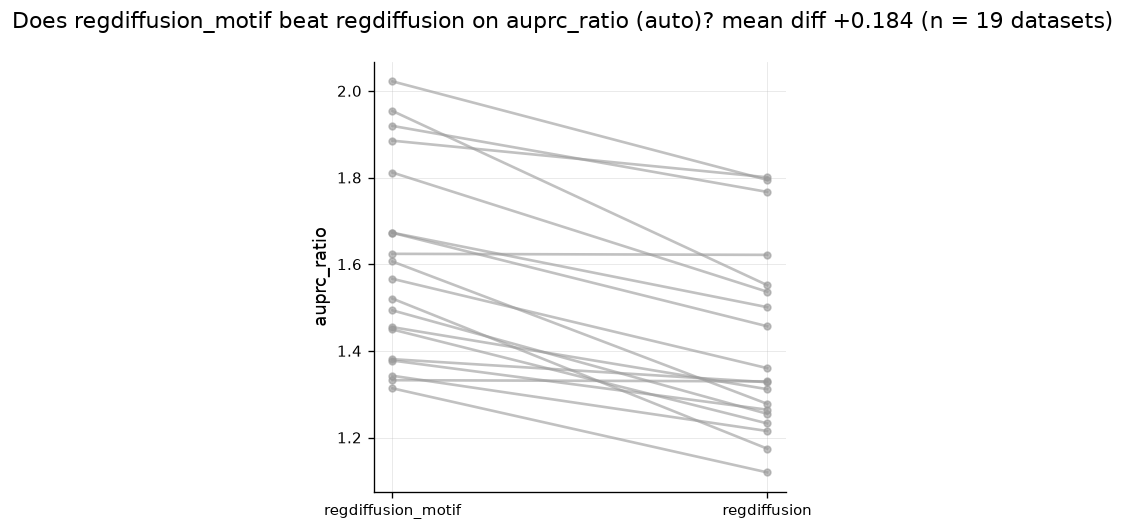
\includegraphics[width=0.85\linewidth]{../viz/lift_regdiffusion_motif_vs_regdiffusion.png}
\caption{-   (n = 19 datasets) - built from  rows/ .json (regdiffusion\_motif vs regdiffusion)}
\end{figure}
\begin{figure}[H]\centering
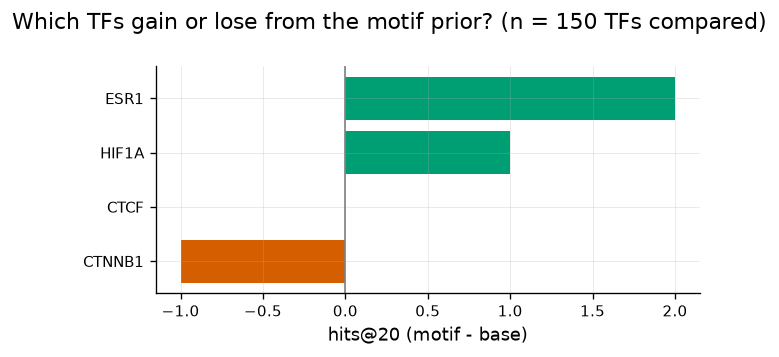
\includegraphics[width=0.85\linewidth]{../viz/motif_lift_cxg__10x-3-v2__homo-sapiens__entorhinal-cortex__06b91002_grnboost2.png}
\caption{-   (n = shared TFs) - built from  grnboost2.tsv.gz vs grnboost2\_motif.tsv.gz}
\end{figure}
\begin{figure}[H]\centering
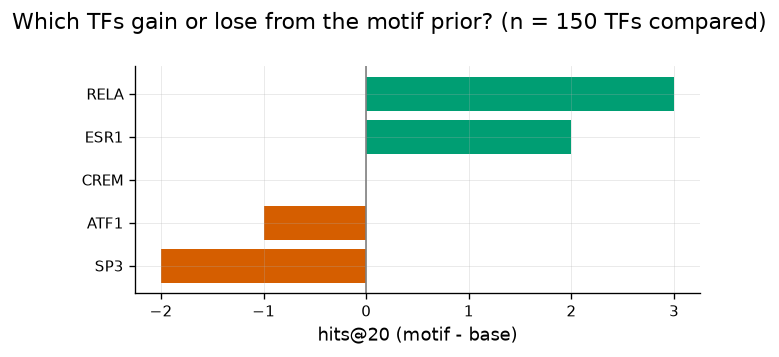
\includegraphics[width=0.85\linewidth]{../viz/motif_lift_cxg__10x-3-v2__homo-sapiens__peripheral-zone-of-prostate__df287f8d_grnboost2.png}
\caption{-   (n = shared TFs) - built from  grnboost2.tsv.gz vs grnboost2\_motif.tsv.gz}
\end{figure}
\begin{figure}[H]\centering
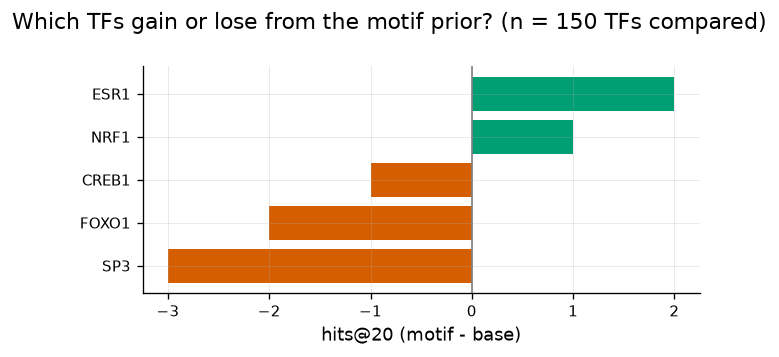
\includegraphics[width=0.85\linewidth]{../viz/motif_lift_cxg__10x-3-v2__homo-sapiens__peripheral-zone-of-prostate__df287f8d_regdiffusion.png}
\caption{-   (n = shared TFs) - built from  regdiffusion.tsv.gz vs regdiffusion\_motif.tsv.gz}
\end{figure}
\begin{figure}[H]\centering
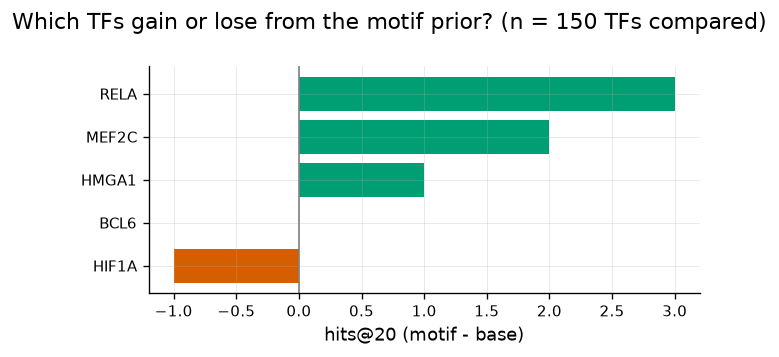
\includegraphics[width=0.85\linewidth]{../viz/motif_lift_cxg__10x-3-v2__homo-sapiens__superior-frontal-gyrus__b94e3bdf_grnboost2.png}
\caption{-   (n = shared TFs) - built from  grnboost2.tsv.gz vs grnboost2\_motif.tsv.gz}
\end{figure}
\begin{figure}[H]\centering
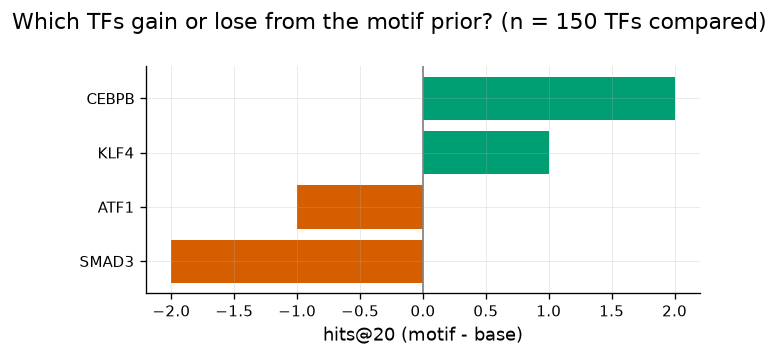
\includegraphics[width=0.85\linewidth]{../viz/motif_lift_cxg__10x-3-v2__homo-sapiens__superior-frontal-gyrus__b94e3bdf_regdiffusion.png}
\caption{-   (n = shared TFs) - built from  regdiffusion.tsv.gz vs regdiffusion\_motif.tsv.gz}
\end{figure}
\begin{figure}[H]\centering
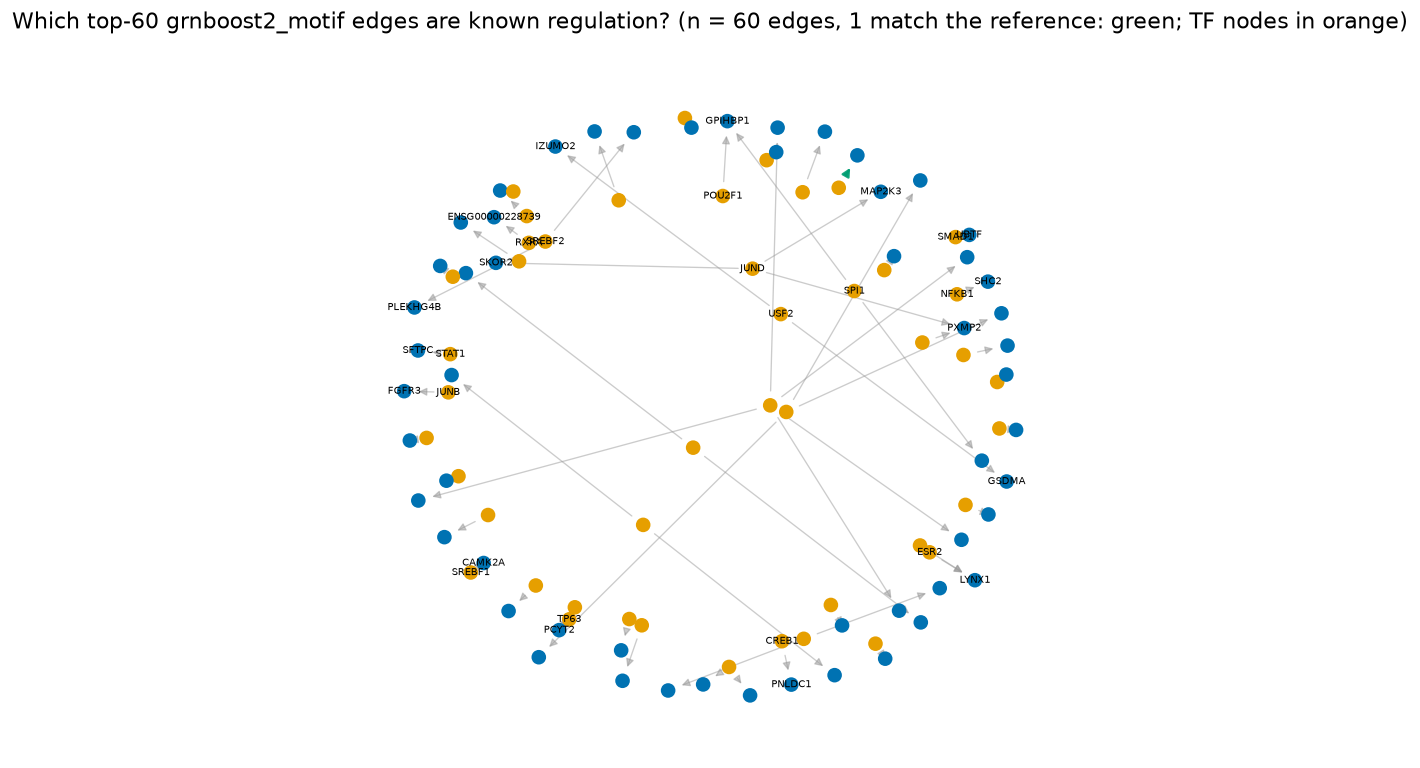
\includegraphics[width=0.85\linewidth]{../viz/network_cxg__10x-3-v2__homo-sapiens__entorhinal-cortex__06b91002.png}
\caption{-   (n = 60 edges) - built from  grnboost2\_motif.tsv.gz}
\end{figure}
\begin{figure}[H]\centering
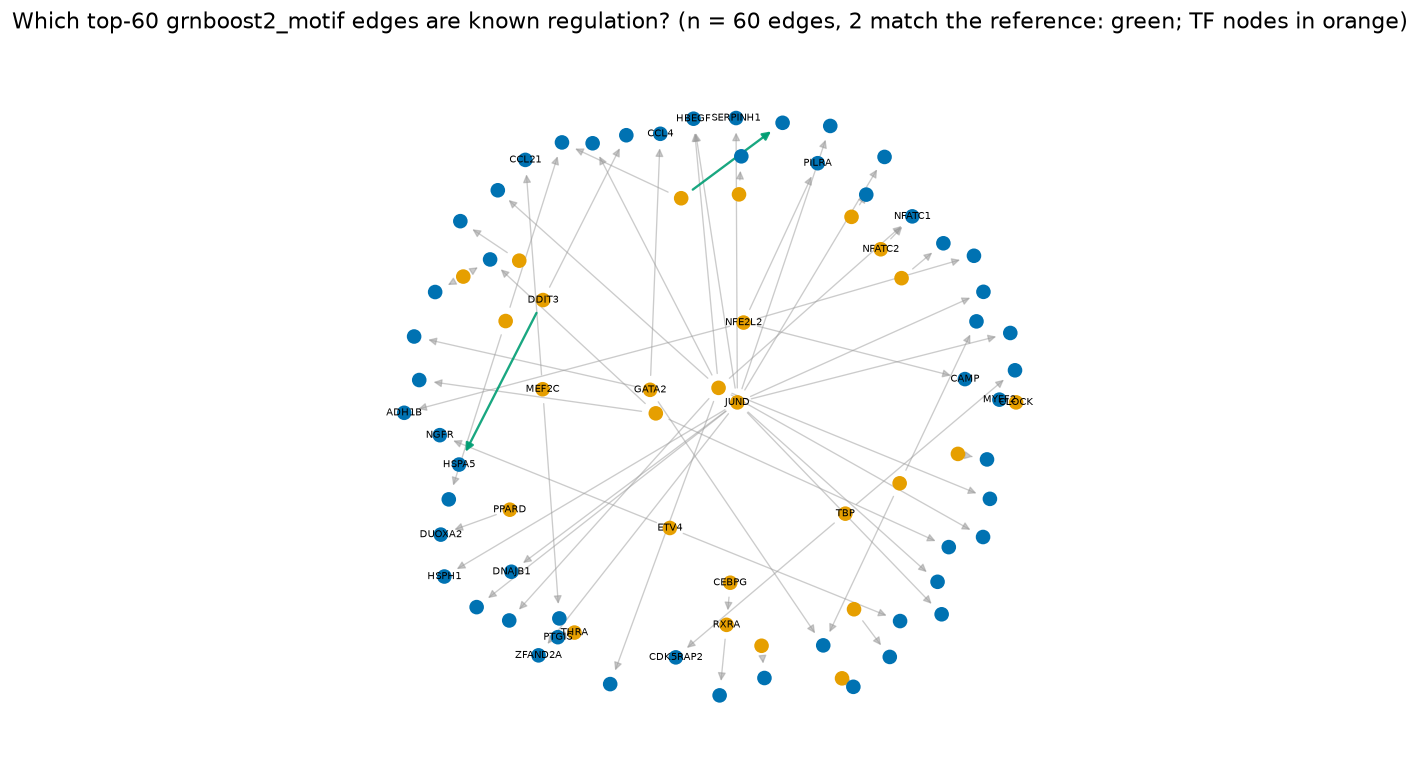
\includegraphics[width=0.85\linewidth]{../viz/network_cxg__10x-3-v2__homo-sapiens__peripheral-zone-of-prostate__df287f8d.png}
\caption{-   (n = 60 edges) - built from  grnboost2\_motif.tsv.gz}
\end{figure}
\begin{figure}[H]\centering
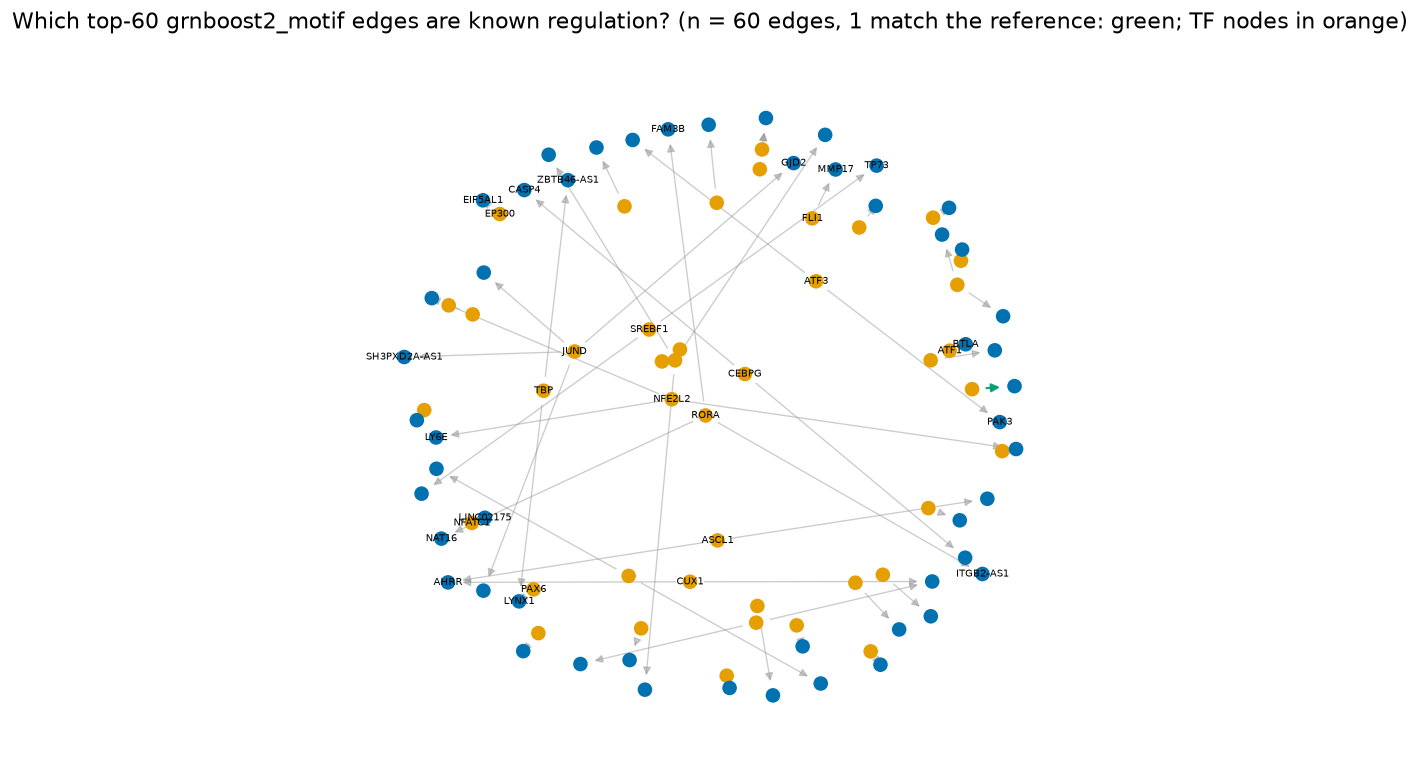
\includegraphics[width=0.85\linewidth]{../viz/network_cxg__10x-3-v2__homo-sapiens__superior-frontal-gyrus__b94e3bdf.png}
\caption{-   (n = 60 edges) - built from  grnboost2\_motif.tsv.gz}
\end{figure}
\begin{figure}[H]\centering
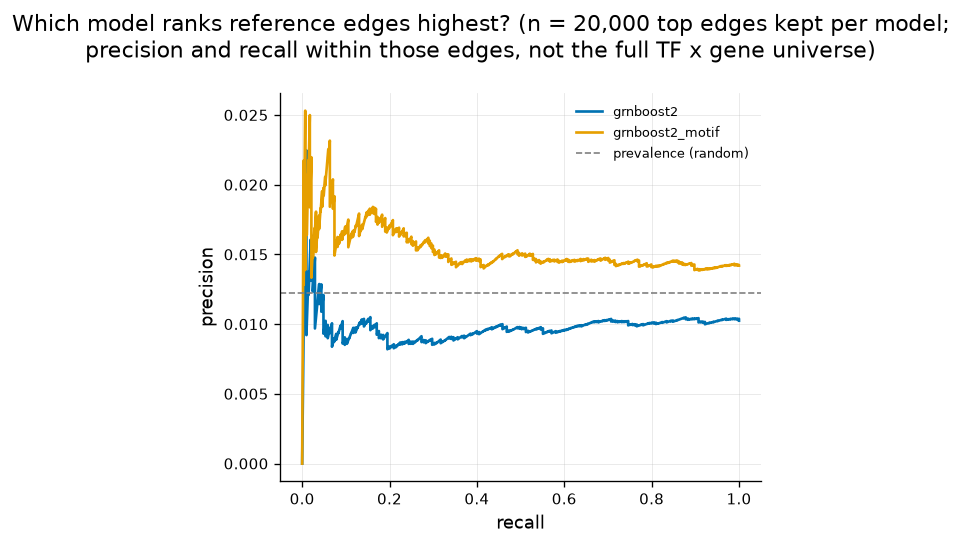
\includegraphics[width=0.85\linewidth]{../viz/pr_cxg__10x-3-v2__homo-sapiens__entorhinal-cortex__06b91002.png}
\caption{-   (n = 20000 edges) - built from  artifacts/cxg\_\_10x-3-v2\_\_homo-sapiens\_\_entorhinal-cortex\_\_06b91002/auto/ctx0}
\end{figure}
\begin{figure}[H]\centering
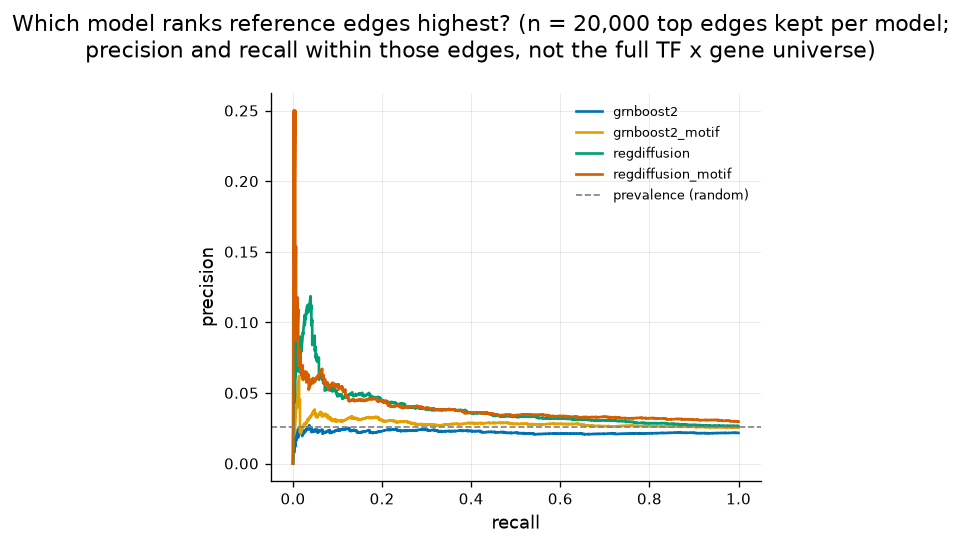
\includegraphics[width=0.85\linewidth]{../viz/pr_cxg__10x-3-v2__homo-sapiens__peripheral-zone-of-prostate__df287f8d.png}
\caption{-   (n = 20000 edges) - built from  artifacts/cxg\_\_10x-3-v2\_\_homo-sapiens\_\_peripheral-zone-of-prostate\_\_df287f8d/auto/ctx0}
\end{figure}
\begin{figure}[H]\centering
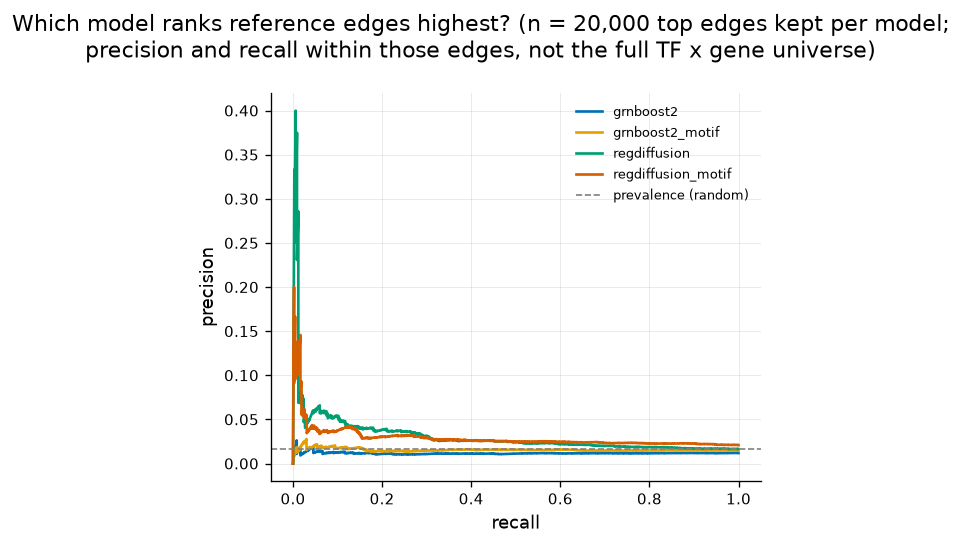
\includegraphics[width=0.85\linewidth]{../viz/pr_cxg__10x-3-v2__homo-sapiens__superior-frontal-gyrus__b94e3bdf.png}
\caption{-   (n = 20000 edges) - built from  artifacts/cxg\_\_10x-3-v2\_\_homo-sapiens\_\_superior-frontal-gyrus\_\_b94e3bdf/auto/ctx0}
\end{figure}
\begin{figure}[H]\centering
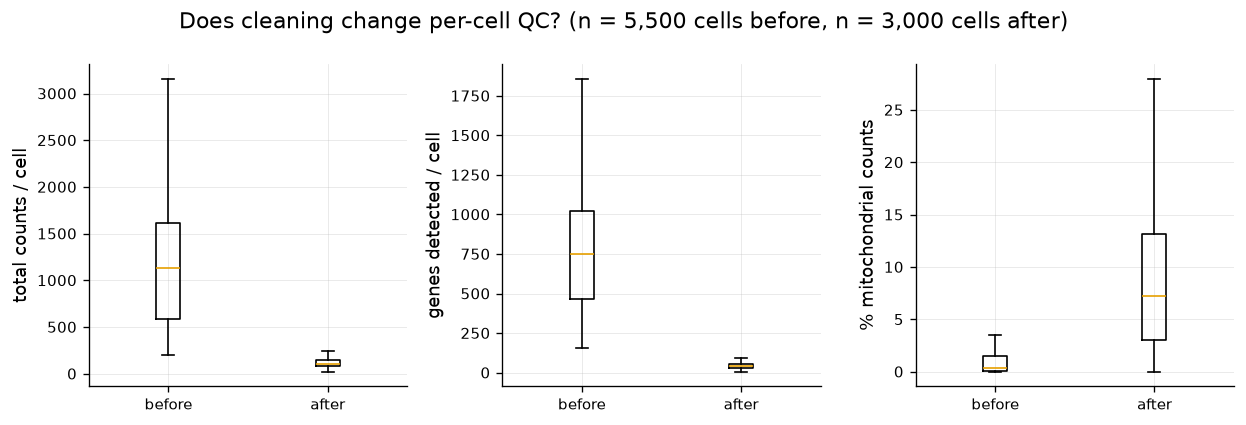
\includegraphics[width=0.85\linewidth]{../viz/qc_cxg__10x-3-v2__homo-sapiens__entorhinal-cortex__06b91002.png}
\caption{-   (n = 5500 cells) - built from  tasks.json (raw data)}
\end{figure}
\begin{figure}[H]\centering
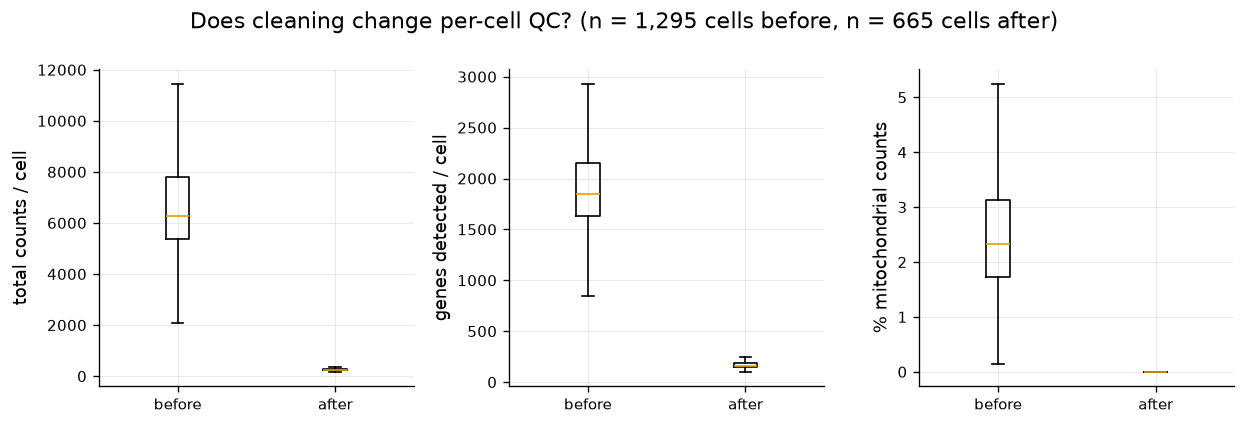
\includegraphics[width=0.85\linewidth]{../viz/qc_cxg__10x-3-v2__homo-sapiens__peripheral-zone-of-prostate__df287f8d.png}
\caption{-   (n = 1295 cells) - built from  tasks.json (raw data)}
\end{figure}
\begin{figure}[H]\centering
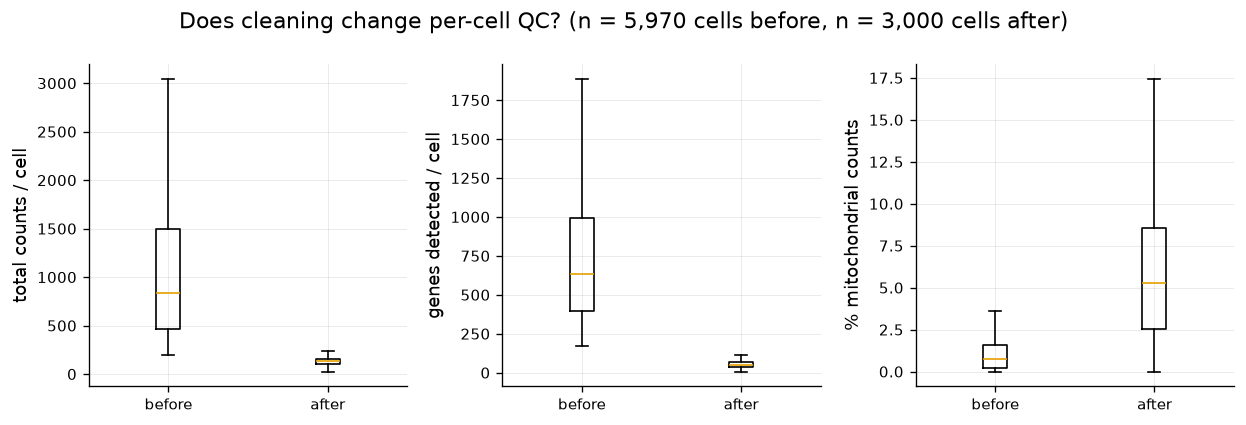
\includegraphics[width=0.85\linewidth]{../viz/qc_cxg__10x-3-v2__homo-sapiens__superior-frontal-gyrus__b94e3bdf.png}
\caption{-   (n = 5970 cells) - built from  tasks.json (raw data)}
\end{figure}
\begin{figure}[H]\centering
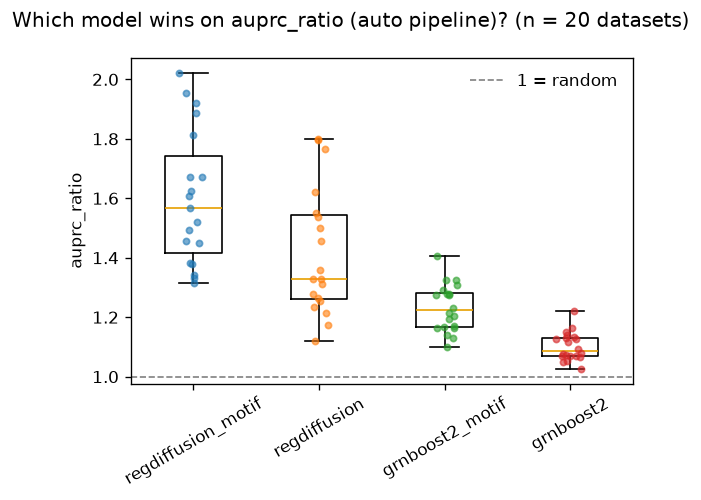
\includegraphics[width=0.85\linewidth]{../viz/scores_auprc_ratio_auto.png}
\caption{-   (n = 20 datasets) - built from  rows/ .json (auto/auprc\_ratio)}
\end{figure}
\begin{figure}[H]\centering
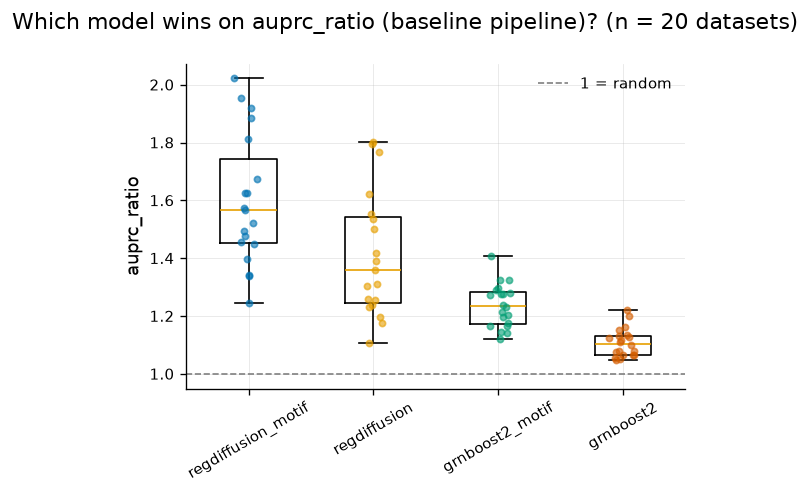
\includegraphics[width=0.85\linewidth]{../viz/scores_auprc_ratio_baseline.png}
\caption{-   (n = 20 datasets) - built from  rows/ .json (baseline/auprc\_ratio)}
\end{figure}
\begin{figure}[H]\centering
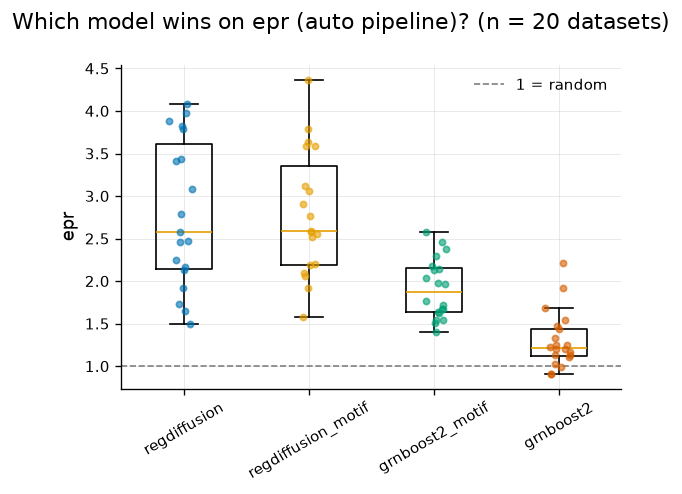
\includegraphics[width=0.85\linewidth]{../viz/scores_epr_auto.png}
\caption{-   (n = 20 datasets) - built from  rows/ .json (auto/epr)}
\end{figure}
\begin{figure}[H]\centering
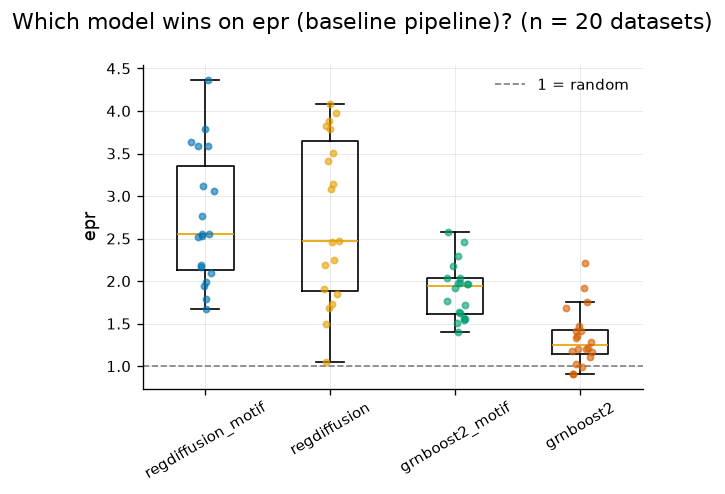
\includegraphics[width=0.85\linewidth]{../viz/scores_epr_baseline.png}
\caption{-   (n = 20 datasets) - built from  rows/ .json (baseline/epr)}
\end{figure}
\begin{figure}[H]\centering
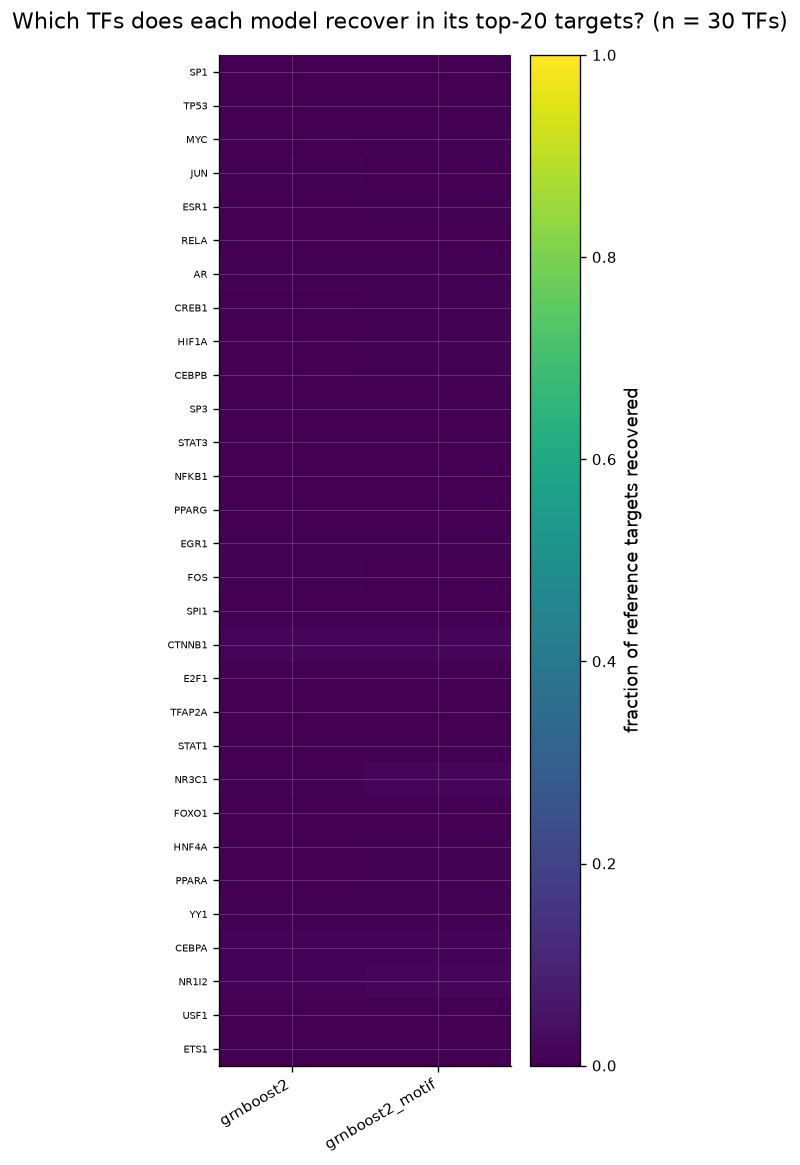
\includegraphics[width=0.85\linewidth]{../viz/tf_recovery_cxg__10x-3-v2__homo-sapiens__entorhinal-cortex__06b91002.png}
\caption{-   (n = up to 30 TFs) - built from  artifacts/cxg\_\_10x-3-v2\_\_homo-sapiens\_\_entorhinal-cortex\_\_06b91002/auto}
\end{figure}
\begin{figure}[H]\centering
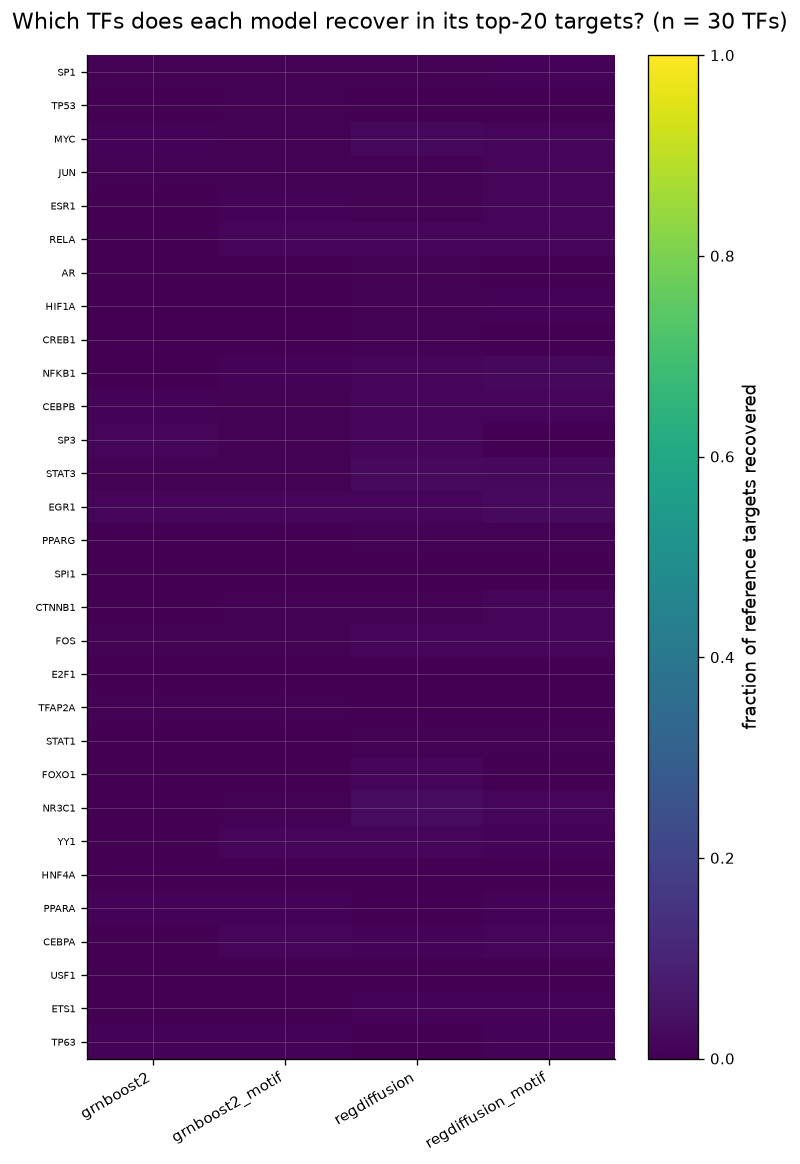
\includegraphics[width=0.85\linewidth]{../viz/tf_recovery_cxg__10x-3-v2__homo-sapiens__peripheral-zone-of-prostate__df287f8d.png}
\caption{-   (n = up to 30 TFs) - built from  artifacts/cxg\_\_10x-3-v2\_\_homo-sapiens\_\_peripheral-zone-of-prostate\_\_df287f8d/auto}
\end{figure}
\begin{figure}[H]\centering
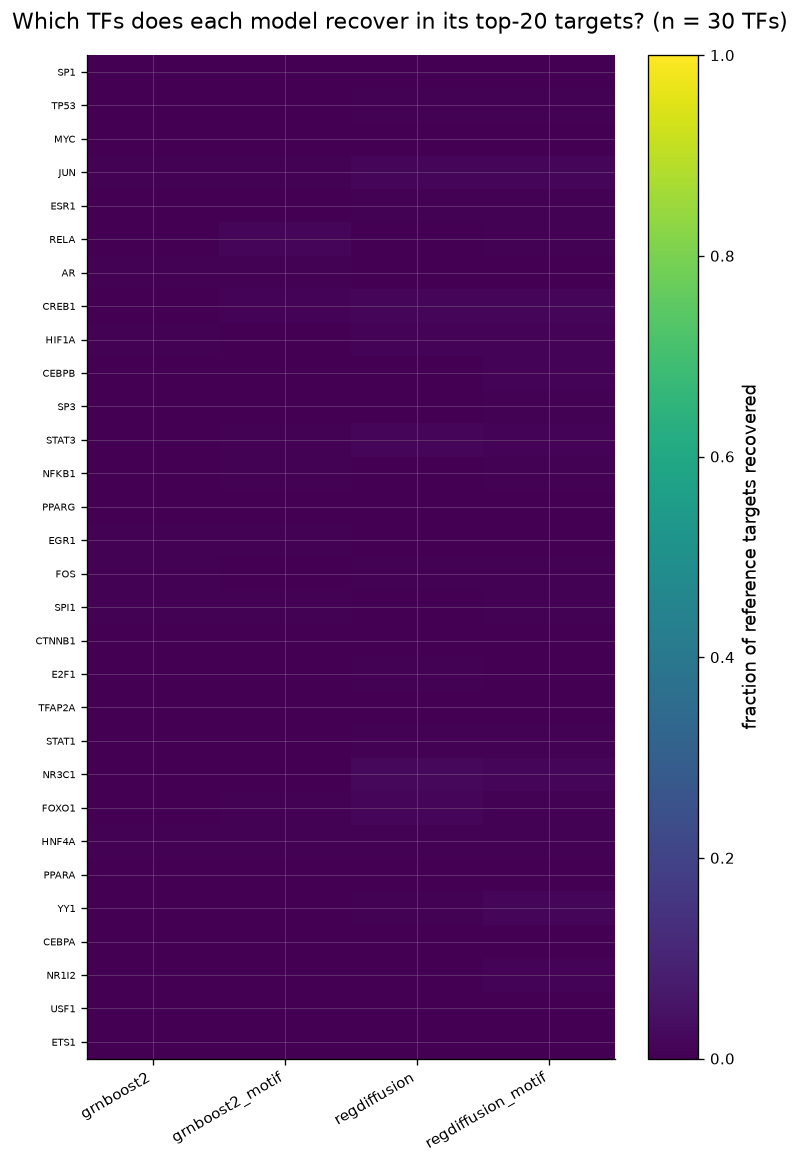
\includegraphics[width=0.85\linewidth]{../viz/tf_recovery_cxg__10x-3-v2__homo-sapiens__superior-frontal-gyrus__b94e3bdf.png}
\caption{-   (n = up to 30 TFs) - built from  artifacts/cxg\_\_10x-3-v2\_\_homo-sapiens\_\_superior-frontal-gyrus\_\_b94e3bdf/auto}
\end{figure}

\section{Limitations}
\begin{itemize}
\item Recorded deviation: deviation 1 above (attempt 1 failed for lack of disk in the compute node's /tmp, one resubmission under rule d); nothing else.
\item Model error in 1 dataset(s): regdiffusion\_baseline.
\item Model error in 1 dataset(s): regdiffusion\_motif\_baseline.
\item Model error in 1 dataset(s): regdiffusion\_auto.
\item Model error in 1 dataset(s): regdiffusion\_motif\_auto.
\end{itemize}

\end{document}
